\documentclass{article}

\usepackage[margin=1in]{geometry}
\usepackage{fancyhdr}
\usepackage{graphicx}
\usepackage{hyperref}
\usepackage{amsmath}
\usepackage{color}
\usepackage{verbatim}


\usepackage{xspace}

\usepackage[margin=1in]{geometry}
\usepackage{listings}
\lstset{language=XML}
\lstset{% general command to set parameter(s)
basicstyle=\footnotesize, % print whole listing small
%basicstyle=\footnotesize, % print whole listing small
keywordstyle=\color{blue}, %\bfseries\underbar,
% underlined bold black keywords
identifierstyle=, % nothing happens
commentstyle=\color{OliveGreen}, % white comments
stringstyle=\ttfamily, % typewriter type for strings
showstringspaces=false, % no special string spaces
language=matlab,
frame=lines,
float=tbfh}

\definecolor{INCFBlue}{rgb}{0.0,0.59,1.0}

\definecolor{issuecolor}{rgb}{0.8,0.8,0.8}
\definecolor{light-gray}{gray}{0.95}
\newcommand{\issue}[1]{%
\begin{center}
\colorbox{issuecolor}{\parbox{0.8\linewidth}{\textbf{Issue:} #1}}
\end{center}%
}

\newcommand{\note}[1]{%
\begin{center}
\colorbox{issuecolor}{\parbox{0.8\linewidth}{\textbf{Note:} #1}}
\end{center}%
}

\newcommand{\suggestion}[2]{%
\begin{center}
\colorbox{issuecolor}{\parbox{0.8\linewidth}{\textbf{#1:} #2}}
\end{center}%
}

\newcommand{\nmlClass}[1]{{\bf #1}}

\newcommand{\ComponentClass}{{\bf{ComponentClass}}\xspace}
\newcommand{\ComponentClasses}{{\bf{ComponentClass}}es\xspace}

\newcommand{\Dynamics}{{\bf{Dynamics}}\xspace}

\newcommand{\MathInline}{\tt{Dynamics}}


\newcommand{\Interface}{{\bf{Interface}}\xspace}
\newcommand{\Interfaces}{{\bf{Interface}}s\xspace}


\newcommand{\StateVariable}{{\bf{StateVariable}}\xspace}
\newcommand{\StateVariables}{{\bf{StateVariable}}s\xspace}


\newcommand{\StateAssignment}{{\bf{StateAssignment}}\xspace}
\newcommand{\StateAssignments}{{\bf{StateAssignment}}s\xspace}


\newcommand{\TimeDerivative}{{\bf{TimeDerivative}}\xspace}
\newcommand{\TimeDerivatives}{{\bf{TimeDerivative}}s\xspace}

\newcommand{\Alias}{{\bf{Alias}}\xspace}
\newcommand{\Aliases}{{\bf{Alias}}es\xspace}

\newcommand{\AnalogPort}{{\bf{AnalogPort}}\xspace}
\newcommand{\AnalogPorts}{{\bf{AnalogPort}}s\xspace}

\newcommand{\EventPort}{{\bf{EventPort}}\xspace}
\newcommand{\EventPorts}{{\bf{EventPort}}s\xspace}

\newcommand{\Port}{{\bf{Port}}\xspace}
\newcommand{\Ports}{{\bf{Port}}s\xspace}

\newcommand{\Event}{{\bf{Event}}\xspace}
\newcommand{\Events}{{\bf{Event}}s\xspace}

\newcommand{\Regime}{{\bf{Regime}}\xspace}
\newcommand{\Regimes}{{\bf{Regime}}s\xspace}

\newcommand{\Transition}{{\bf{Transition}}\xspace}
\newcommand{\Transitions}{{\bf{Transition}}s\xspace}

\newcommand{\Trigger}{\tt{Trigger}}

\newcommand{\OnEvent}{{\bf{OnEvent}}\xspace}
\newcommand{\OnEvents}{{\bf{OnEvent}}s\xspace}

\newcommand{\OnCondition}{{\bf{OnCondition}}\xspace}
\newcommand{\OnConditions}{{\bf{OnCondition}}s\xspace}


\newcommand{\Parameter}{{\bf{Parameter}}\xspace}
\newcommand{\Parameters}{{\bf{Parameter}}s\xspace}


\newcommand{\OutputEvent}{{\bf{OutputEvent}}\xspace}
\newcommand{\OutputEvents}{{\bf{OutputEvent}}s\xspace}


\newcommand{\SendPort}{{\tt{SendPort}}\xspace}
\newcommand{\RecvPort}{{\tt{RecvPort}}\xspace}
\newcommand{\ReducePort}{{\tt{ReducePort}}\xspace}
\newcommand{\SendPorts}{{\tt{SendPorts}}\xspace}
\newcommand{\RecvPorts}{{\tt{RecvPorts}}\xspace}
\newcommand{\ReducePorts}{{\tt{ReducePorts}}\xspace}

\begin{document}

\pagestyle{empty}

\begin{center}
{
\includegraphics[width=0.7\columnwidth]{images/incf.png}}
\end{center}

\vspace*{1cm}

\noindent\rule{\columnwidth}{1pt}
\noindent\rule{\columnwidth}{2pt}

\vspace*{1cm}

\begin{center}
\noindent{\Huge \bf Network Interchange for Neuroscience Modeling Language
(NineML)}\\
\vspace{0.5cm}
\noindent{\Large \bf Specification}\\
\vspace{0.5cm}
\noindent{\large INCF Task Force on Multi-Scale Modeling}\\
\vspace{0.5cm}
\noindent{\large Version: 0.98-1}
\end{center}

\vspace*{0.75cm}

\noindent\rule{\columnwidth}{2pt}
\noindent\rule{\columnwidth}{1pt}

\vspace*{3cm}
\noindent{\Large

\begin{center}
{\bf Written by: }
\end{center}

\noindent Anatoli Gorchetchnikov, Ivan Raikov, Mike Hull, Yann Le Franc  \\

%\vspace*{0.5cm}

\noindent {\bf Date:} \today

}

Acknowledgements: We would like to thank the Task Force members for their
comments on this document and in particular P. Gleeson, E. Muller, A. Davison,
R. Cannon, S. Hill.

\title{NineML (9ML) Specification}

\newpage
\pagestyle{plain}

\newpage

\abstract
NineML is a simulator independent language with the aim of providing an
unambiguous description of neuronal network models for efficient model sharing
and reusability. This language emerges from a joint effort from experts in the
field of Computational Neuroscience, simulator development and standardized
language initiative (NeuroML), coordinated and supported by INCF.

This document provides the basis for understanding the Common Object Model,
shared by the three  implementations, and the resulting XML schema and tags. The
current work only covers the representation of spking neurons and synapses and
will be further extended to represent network connectivity, synaptic plasticity,
and all other necessary concepts to represent networks.
These extensions are still work in progress and your comments and feedbacks will
be extremely valuable.

\newpage
\tableofcontents

\newpage
\vskip 1in
\paragraph{Changes from version 0.98:}
\begin{itemize}
\item Text edition and reorganization of the document.
\item Description of the OM classes are reorganized to ``fit'' the hierarchical
structure in XML both for the AL and the UL.
\end{itemize}

\paragraph{Changes from version 0.97:}
\begin{itemize}
\item Using math mode for math expressions; consistent type faces for
  class names; small tweaks to the MathInline definition; moved Scope
  section (5.1) to an appendix (Ivan Raikov)
\end{itemize}

\paragraph{Changes from version 0.96:}
\begin{itemize}
\item Draft definition of MathInline block (Mike Hull)
\end{itemize}

\paragraph{Changes from version 0.95:}
\begin{itemize}
\item Moved section Transition Resolution to the Appendix; consistent
  highlighting of NineML class names (Ivan Raikov)
\end{itemize}

\paragraph{Changes from version 0.94:}
\begin{itemize}
\item Merged in Abstraction Layer documentation by Mike Hull
\end{itemize}

\paragraph{Changes from version 0.93:}
\begin{itemize}
\item Combined User and Abstraction Layer specifications into a single document
\item Cut out the group and set sections since they are not part of the release
\end{itemize}

\paragraph{Changes from version 0.92:}
\begin{itemize}
\item Adapted the format similar to the Abstraction layer specification.
I think this document shall essentially become User Layer section of the
general specification document.
\item Attempted to reorganize and adapt the text to be more like ``Object
Model'' for the User Layer.
\end{itemize}

\paragraph{Changes from version 0.91:}
\begin{itemize}
\item Replaced ``node'' with ``component'' as was decided in Antwerp 2010
meeting.
\item Replaced references to ``core semantics'' with references to
``Abstraction Layer'' because the term ``core semantics'' is no longer used.
\item As Antwerp 2010 decided, properties are represented by a generic
tag and specified by attribute {\tt name}.
\item Added the reference to units of measurements dimensionality checking
against the Abstraction Layer as was decided in Antwerp 2010.
\item Moved edge effect descriptions from connectivity components to layout
components. Also noted that some layouts might require complex masks.
\end{itemize}

\paragraph{Changes from version 0.9:}
\begin{itemize}
\item added footnotes for some issues raised in Stockholm June meeting
\item added brief description of interactions between User Layer and
simulation software that does not support Abstraction Layer
\item removed random number generator nodes as decided in Stockholm
\item added space, region, and layout nodes as a first draft of geometrical
concepts (based on NetworkML proposal by Padraig and Robert as well as
Stockholm discussions)
\item removed recurrent projections that can be described on the population
level
\item cut out the previous approach to cell positioning within population
\end{itemize}
\newpage

\section{Introduction}

The increasing number of studies related to neuronal network modeling and the
diversity of the simulation platforms and implementations cause a major issue
for model sharing, replicability and reusability of either whole model or part
of the model for further analysis or simply for extension.
To overcome this problem, we are proposing a common description language to be
used for exchanging models and being able to simulate them in any simulation
platform.
This description language, using the XML technology, is based on a common Object
Model describing the different elements of network models. This work, initiated
and supported by the International Neuroinformatics Coordinating Facility as
part of the MultiScale Program, involve simulator developers and developers from
NeuroML, a similar initiative.
The name of the proposed language is NineML (Network Interchange for
Neuroscience Modeling Language).

\subsection{Scope}

The purpose of NineML is thus to provide a computer language for
succinct and unambiguous description of computational neuroscience models of
networks of spiking neurons.

NineML is intended to describe the network architecture, parameters
and equations that govern the dynamics of a network of spiking
neurons, without taking into account model implementation detail such as
numerical integration method.

At the current stage of development, the following concepts of spiking neuron
network modeling can be fully or partially described:

\begin{enumerate}
\item spiking neurons
\item synapses
\begin{enumerate}
\item Post-synaptic membrane current mechanisms
\item Short-term synaptic dynamics (a la Markram et. al. 1998)
\item Long-term synaptic modifications (STDP, learning, etc.)
\end{enumerate}
\end{enumerate}

The Object Model developped has been used to create three different
implementations (Java, Python and Chicken Scheme) that are now able to
import/export a common XML description and generate code for simulating the
described model in different simulator.

\subsection{Design Considerations}

As one of the goals of NineML is to provide a mean to import/export a model from
any simulator or implementation, it is crucial to maintain a clear distinction
between the definition of NineML and a simulator. Therefore, NineML should
provide only the information necessary for any given simulator
to instantiate the network models in a simulator agnostic way.
For example, NineML should specify the neuron membrane equation to solve,
but not how to solve it.  In addition, for implementation and performance
reasons, it is important to keep the language layer ``close'' to the simulator –
such that the language layer is not responsible for maintaining separate
representations of the instantiated network. [COMMENT\_YANN: WHAT DO YOU MEAN??]

A NineML object model representation can take multiple forms.  A
program can employ a concrete representation of the NineML objects in
a specific programming language, or it can convert an internal model
representation to and from the NineML XML schema, or it can take the
form of an interpreter for the NineML native language as a compact
representation and use code generation to produce a model
representation for a target simulation environment.

The design of NineML is divided into two semantic layers:
\begin {enumerate}
\item \underline {an Abstraction Layer} that provides the core concepts and
mathematical descriptions with which
model variables and state update rules are explicitly described in {\em
parametrized} form, and
\item \underline {a User Layer} that provides a syntax to specify the
instantiation and the value of parameters of all these components of a network
model.
\end {enumerate}

As the User Layer provides the mechanism for instantiating and parameterization
of the model elements that have been defined in the Abstraction Layer, it is
clearly essential that these two layers share a complementary and compatible
design philosophy. There must be a clear definition of which aspects of a model
are defined in the User Layer and which are defined in the Abstraction Layer.
In addition, the mechanisms for naming and addressing Abstraction Layer concepts
that are instantiated in the User Layer have been kept simple for the user.

\subsection{About this document}

This document presents the current NineML specifications and consists of:
\begin{enumerate}
\item a description of the Abstraction and User Layer Object models
\item the XML serialization with the description of the different tags
\item examples of XML descriptions
\end{enumerate}

It is important to note that the NineML XML schema is isomorphic to the NineML
object model.

\section{Abstraction Layer: Core Concepts }
\label{AbstractionL}

[TO DO: Here a introduction to the AL with the description of the graph
approach.]
The Abstraction Layer aims at providing general concepts to represent the
mathematical entities defining the dynamics of the different types of models
composing a network (neuron models, synapse models, synaptique/intrinsic
plasticity, ...)
The Object Model for the Abstraction Layer has been developed using a graphical
representation of the different components and their inter-relations.
This type of representation allows to visualize the interactions between the
different components of a particular type of model and presents clear heuristic
"properties".
We will use this graph representation to introduce the core concepts of the
Object Model.

\subsection{ComponentClass}

\begin{figure}[htb!]
\center
\includegraphics[width=8cm]{figures/component_simple.pdf}
\protect\caption{ComponentClass Overview (Simple)\ref{code:xmliz}}
\label{fig:EX1_RegimeGraph}
\end{figure}

The main building block of the Object Model is the ComponentClass.
It is designed to represent all the individual entities existing in a network
model (cells, synapses, synaptic plasticity rules, random spike train, inputs,
...).
A \ComponentClass is the conglomerating object which is the subject of
interaction with the User Layer and is composed of a \Dynamics block and
\Interfaces to communicate between each other.

[TO DO: Here should be a graph representing the ComponentClass and showing
Dynamics and Interfaces]

[MIKE'S COMMENT: IT MAKES THINGS MORE CONFUSING. Want to know the core ideas
without implementation details...examples provide the information about the
implementation]
This concept is mapped with the following XML tag:

\begin{lstlisting}[frame=none, backgroundcolor=\color{light-gray}]
<ComponentClass name="">
	...
</ComponentClass>
\end{lstlisting}

Example:
\begin{lstlisting}[frame=none, backgroundcolor=\color{light-gray}]
<ComponentClass name="izhikevichCellNew">

... here you will detail parameters, equations, ...

</ComponentClass>
\end{lstlisting}

\subsection{Interfaces}

The interface is the \emph{external} view of the component that defines
what inputs and outputs the component exposes to other components and the
parameters that can be set for the component. The interface consists of
instances of \Port (section~\ref{ports}) and \Parameter
(section~\ref{parameters}).

As well as being able to communicate continuous values, components are also
able to emit and receive \Events. Events are discrete notifications
that are transmitted over \EventPorts (section~\ref{eventPorts}). Since
\EventPorts have names, saying that we transmit 'event1' for example
would mean transmitting an event on the EventPort called 'event1'. Events
can be used to signal action potentials firing for example.

\subsubsection{Parameter}

Parameters corresponds to a placeholder for a numerical value with or without
dimensions, defining particular aspects of the model, such as the firing
threshold, reset voltage, the decay time constant of a synapse model.
The instantiation of Parameters at the Abstraction Layer level allow us to
define the dynamics of a component once, then adjust the behaviours by using
different parameters.  [TO DO : modify text. Better to talk about a general
canvas or unique representation of the dynamics]
For example, if we are building an integrate-and-fire neuron, we can specify
that the
Reset-Voltage and the Firing-Threshold are parameters, write our
dynamics in terms of these parameters, then use the User Layer to
provide parameters to create different neurons. By definition, Parameters are
set at the start of the simulation, and remain constant throughout.

\subsubsection{Port}

Ports allow components to communicate between each other during a simulation.
There are two sub-classes of \nmlClass{Port} objects: \nmlClass{AnalogPort}
and \nmlClass{EventPort}, and each can have different modes.

%\subsubsection{AnalogPort}
\paragraph{AnalogPort}

AnalogPorts transmit and receive continuous values, either \Alias
or \StateVariable. \AnalogPort can have 3 modes:
\begin{itemize}
\item \SendPort - transmit data originating in this component which can
be read by other components.
\item \RecvPort - receive data from another components \SendPort
port. Each \RecvPort can be connected to \emph{one} \SendPort.
\item \ReducePort - receive data from multiple \SendPorts. These
differ from \RecvPorts in that they can be connected to multiple
\SendPort. \ReducePorts take an additional operator,
{\tt reduce\_op}, which specifies how the data from multiple \SendPorts
should be combined to produce a single value. Currently, the
only supported operations is $+$, which sums the inputs.
The motivation for \ReducePort is that it allows us to make our
component definitions more general. For example, if we are defining a
neuron, would define a \ReducePort called {\tt InjectedCurrent}.
This allows us to write the membrane equation for that neuron as
$dV/dt = (1/C) * InjectedCurrents$.

Then, when we connect this neuron to synapses, current-clamps, etc, we
simply need to connect the SendPorts containing the currents of these
components onto the {\tt InjectedCurrent} reduce-port, without having
to change our original component definitions.
\end{itemize}

%\subsubsection{EventPort}
\paragraph{EventPort}

\label{eventPorts}

Event ports transmit discrete events. They are useful for example in
simulation of integrate-and-fire neurons to notify components about neuron's
spiking. Event ports only have 2 modes:

\begin{itemize}
\item \SendPort - transmit events originating in this component which can be
read by
other components
\item \RecvPort - receive events from another components \SendPort port.
Each recv port can be connected to \emph{multiple} \SendPorts.
\end{itemize}

For example, a synapse component may have a \RecvPort connected to the
presynaptic neurons \SendPort port. When the presynaptic neuron fires;
it delivers an event to the synapse, which could cause it to produce current
flow in a post-synaptic neuron.

\subsection{Dynamics}

The \Dynamics block represents the \emph{internal} mechanisms governing the
behaviour
of the component.
For most of the models these dynamics are non-linear, presenting transitions
between different regimes at particular values of one or different state
variables.
To create a representation that include both simple dynamics and non-linear
dynamics, the \Dynamics block can contains the following concepts:

\begin{itemize}
\item \StateVariable (section~\ref{state-var})
\item {\tt Regime(s)} (section~\ref{regime}) that describe the dynamic of the
system for particular values of \StateVariable
\item Transition(s) links two regimes and the condition
\item \Alias (section~\ref{alias})
\end{itemize}

These different concepts are the building blocks of a graph, called the {\tt
Regime Graph} (illustrated in figure ?), where the \Regime forms the vertices
and the \Transition form the directional edges of the {\tt Regime Graph}.
This graph must have at least one \Regime, and contain no regime islands.  At
any given time, a
component will be in a single \Regime, and can change which \Regime it is in
through \Transition.

\begin{figure}[htb!]
\center
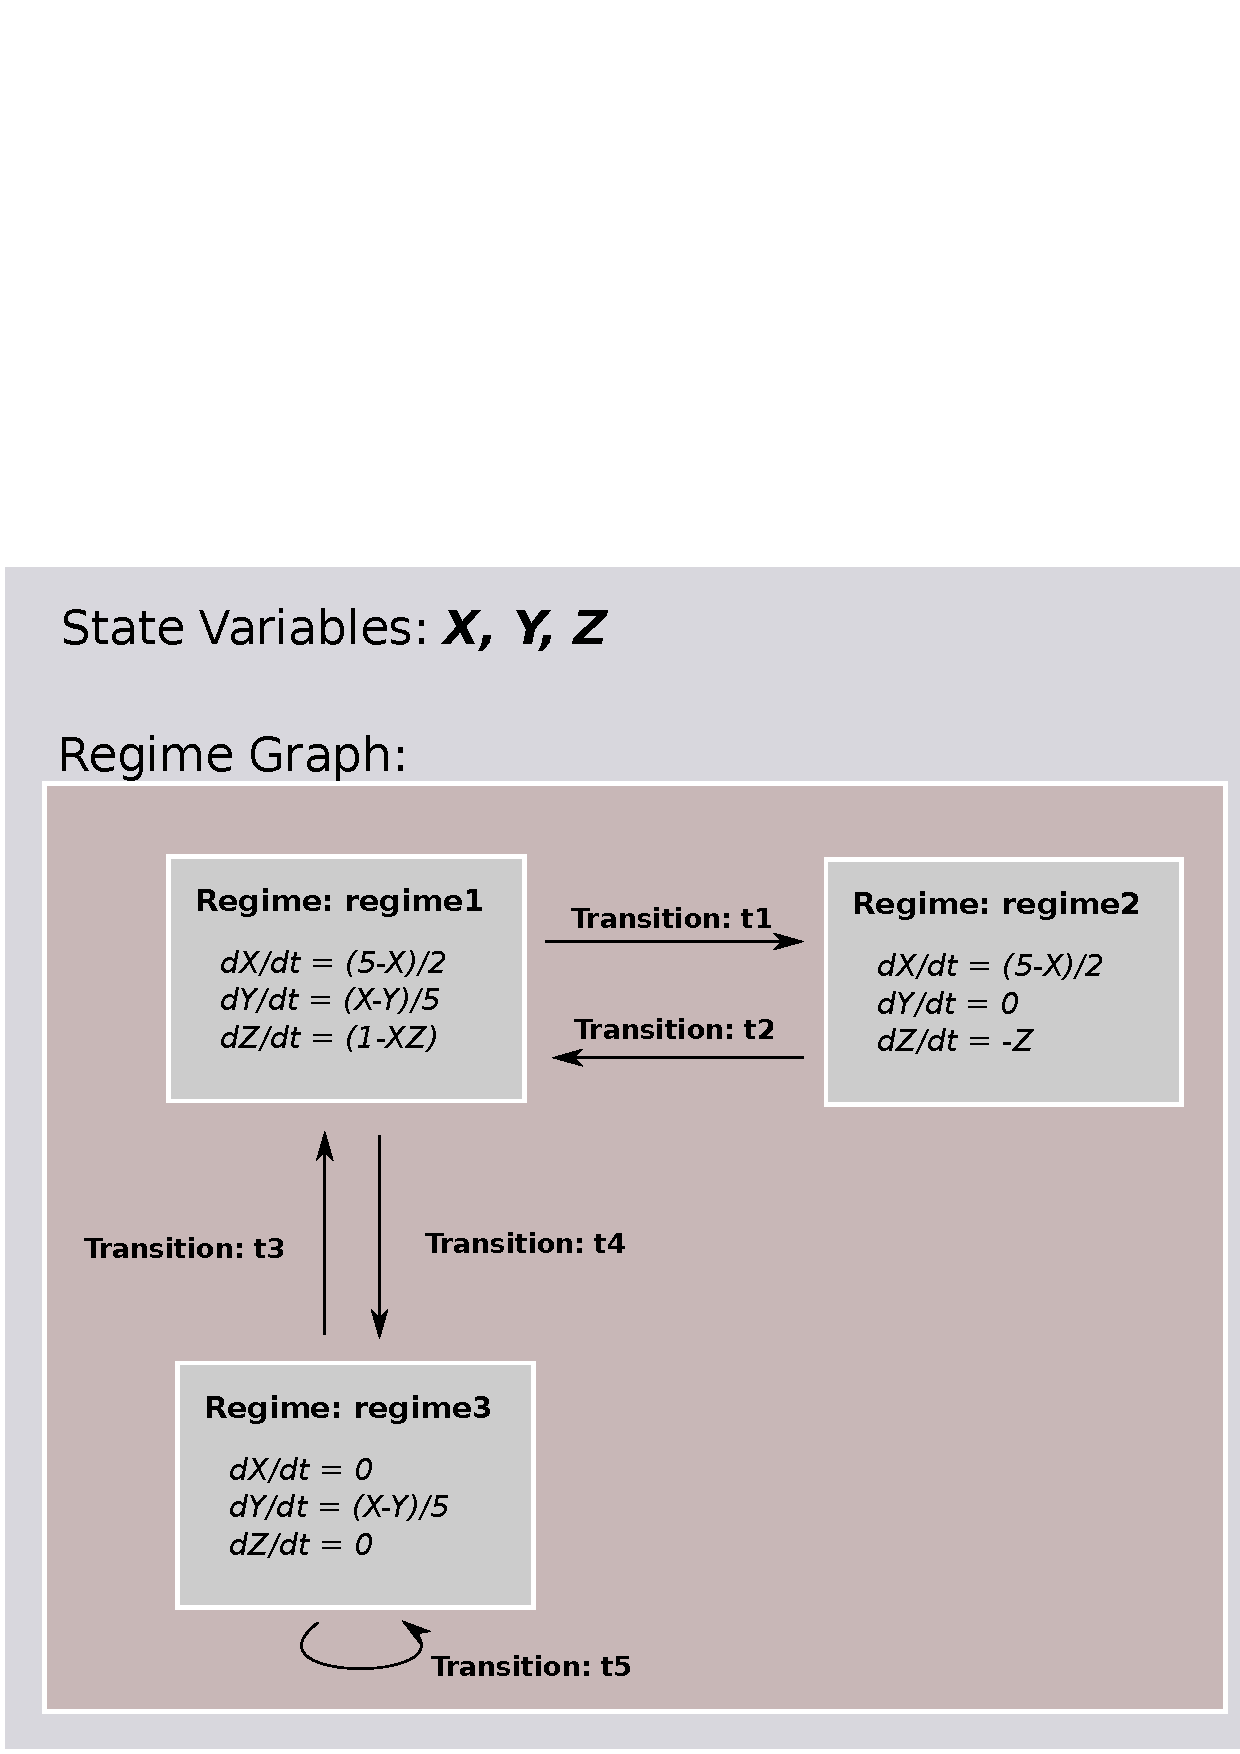
\includegraphics[width=14cm]{images/SimpleRegimeGraph.png}
\protect\caption{The dynamics block for an example component.}
\label{SimpleRegimeGraph}
\end{figure}

An example dynamics in Figure~\ref{SimpleRegimeGraph} has three state variables,
\emph{X,Y} and \emph{Z}, and a state graph with three regimes, \emph{regime1},
\emph{regime2} and \emph{regime3}. At any time, a component will be in one of
these regimes, and the state variables will evolve accordingly.

\subsubsection{StateVariable}

The internal state of a component is defined by a set of \StateVariable
-- variables that can change either continuously or discontinuously as a
function of time.

The \StateVariable changes happen in two ways:
%
\begin{quote}
\begin{itemize}
\item continuously through \textbf{TimeDerivatives} (in \Regimes),
which define the \StateVariables evolution over time, for example
$dX/dt=1-X$.
\item discretely through \StateAssignment (in \Transition),
which make discrete changes to a \StateVariable value, for example
$X = X + 1$.
\end{itemize}
\end{quote}

\subsubsection{Regime}

A \nmlClass{Regime} is defined in NineML as a system of ODEs in time
on \StateVariable.  As such, \Regime defines how the \StateVariables change
(propagate in time) between subsequent \Transitions. \Regime is defined to have
non-vanishing
temporal extent. Once construction of the \Regime is complete, it
should have defined the following properties:

\begin{itemize}
\item An unordered collection of \nmlClass{StateVariable}s which are
propagated when the \nmlClass{Regime} is active.
\item a set of \TimeDerivative, one for each \StateVariable
of the \ComponentClass, which define how the \StateVariable
evolve over time in the form $\frac{dx_{i}}{dt} = f(x\_0, ..., x\_i, t)$.
\item \Parameter for the \nmlClass{Regime}
\item An unordered collection of \nmlClass{AnalogPort}s which publish state
variables (type=send), or consume state variables published from elsewhere
(type=recv, or type=reduce).
\item The independent variable must be shared between the collection
of \StateVariables and their propagators in a Regime.
\end{itemize}

\note{If a \textbf{TimeDerivative} for a \StateVariable is not defined
in a \Regime, it is assumed to be zero.}

It is important to note that, at the current stage of development, we are only
considering "Temporal regimes". In the next version, we will extend the concept
to the more general case where the independent variable can be anything (space
for example)

[TODO:
Sean's comment:
We should not preclude other systems of equations,
overrideing regime, spatial regimes ...

Generalize ODEs to general propagators ...
ODE is a special case of a propagator ...
Independent variable
Who: Ivan.
]

[TODO: Hybrid state machine as Appendix to clearly define Regime
in terms of atomic lower-level primitives.
Who: Ivan
]

[TODO:
TemporalRegime vs Regime ...
For this Developer release, Regimes are Temporal Regimes.
Who: not assigned until after CNS
]

\subsubsection{Condition}

\nmlClass{Condition}s are the mathematical expressions which define
when a \nmlClass{Transition} should be triggered.
\nmlClass{Condition}s are any arbitrary combination of \emph{Logical
Operations} (and, or, noop, etc.) on the
result of any arbitrary combination of \emph{Relational Operations}
($>$,$<$,$==$,$<=$,$>=$, etc.) on
\nmlClass{StateVariable}s. At any given time in the \nmlClass{Regime},
the \nmlClass{Condition} expression then evaluates to True or False
{\tt Boolean} result. For example, the following are valid
\nmlClass{Condition}s

\begin{verbatim}
x>10
x>10 & y<20
x>exp(-cos(y)) | y<sin(t)+5
x==15
\end{verbatim}

A \nmlClass{Condition} which persistently evaluates to True
violates the definition that \nmlClass{Tranisiton}s should have vanishing
temporal extent, and the behaviour for this case is undefined, but
it would be preferable for the implementation to produce an error
message to the user.

\subsubsection{Transition}

Movement between several instances of \Regime happens via \Transition.
A \nmlClass{Transition} is defined in NineML as having
a source and target \nmlClass{Regime}, where the target
\nmlClass{Regime} can be the same as the source (For example \emph{t5}
in Figure~\ref{SimpleRegimeGraph}). There are two types of \Transition:

\begin{itemize}
\item An \OnCondition function of the \StateVariable, for
example $X > Y$.
\item An \OnEvent on an input from \EventPort. (Discussed in
sections~\ref{events} and \ref{eventPorts}).
\end{itemize}

During either type of transition three things can happen:
\begin{itemize}
\item The component can change regime. For example, if
the component is in \emph{regime3}, and the trigger for \emph{t3} is
satisfied, then the component will move into \emph{regime1}.
\item \textbf{StateAssignment}s can take place, for example, $X=0$
\item The component can send \OutputEvent
\end{itemize}

During a transition, multiple \StateAssignment and \OutputEvent can occur.
(For more on the resolution of \Transition, see section~\ref{resolution})

\nmlClass{Transition}s have a vanishing temportal extent (i.e. they are
event-like). Once construction of a \nmlClass{Transition} is complete, it
should have defined the following properties:
\begin{itemize}
\item The \nmlClass{Condition} or \nmlClass{EventPort(mode=recv)} which
triggers the \nmlClass{Transition}
\item An set of \StateAssignment and\OutputEvent objects
\item The label of the source \nmlClass{Regime}, and the label of the target
\nmlClass{Regime}, which may be the same as the source \nmlClass{Regime}.
\end{itemize}

\subsubsection{Aliases}

An alias correspond to an intermediate variable allowing to store an information
and to reuse it at different places in the definition of the dynamics. [TO DO:
rewrite to incorporate the term substitution and make the definition clearer]

\textbf{Aliases} are motivated from two problems:

\begin{itemize}
\item Rather than writing long expressions for functions of \StateVariable,
we can define an \Alias once. For example, we can define chains of
\Aliases:
%
\begin{quote}{\ttfamily \raggedright \noindent
m\_alpha~=~(alphaA~+~alphaB*V)~/~(~alphaC~+~exp((alphaD+V/alphaE))~)\\
m\_beta~=~~(betaA~+~betaB*V)~/~(~betaC~+~exp((betaD+V/betaE))~)\\
minf~=~m\_alpha~/~(m\_alpha~+~m\_beta)\\
mtau~=~1./(m\_alpha+m\_beta)\\
dm/dt~=~(1/C)~*~(minf-m)/mtau
}
\end{quote}

In this case, $m_{alpha}$, $m_{beta}$, $minf$ and $mtau$ are all
alias definitions. There is no reason we couldn't expand our $dm/dt$
description out to eliminate these intermediate \Aliases, but the expression
would be very long and difficult to read.

\item If we would like to communicate a value other than a simple \StateVariable
to another \ComponentClass. For example, if we have a component representing a
neuron, which has an internal \StateVariable, 'V', we may be interested in
transmitting a current, for example $i=g*(E-V)$.
[TO DO: add the fact that an alias is required for passing values through the
Port]

\end{itemize}

\note{\Alias is defined in the Dynamics, \emph{not} in the
\Regime. This means that aliases are the same across all regimes.}

\subsection{To summarize}

\begin{figure}[htb!]
\center
%\includegraphics[width=14cm]{al/ParallelisingTransitions.pdf}example_IzRegimeTransGraph.pdf
\includegraphics[width=0.9\linewidth]{figures/component_complex.pdf}
\protect\caption{ComponentClass Overview (Detailed)\ref{code:xmliz}}
\label{fig:EX1_RegimeGraph}
\end{figure}

\newpage

\section{User Layer: Core Concepts}
\label{UserL}

\subsection{Component}

The basic building block of NineML User Layer is called component. In the
User Layer description component is a reference to a \ComponentClass
object defined in the Abstraction Layer. Abstraction Layer defines the
mathematics of the component and this definition is then referred in the
User Layer through an object of type {\tt Definition}.

\begin{table}[htb]
\center
\begin{tabular}{|c|}
\hline
\hline
Component \\
\hline
\hline
{\em label}: {\tt String} \\
\hline
{\em definition}: \{{\tt Definition}$|${\tt Reference}\}\\
\hline
{\em note}: \{{\tt String}$|${\tt URL}\} (optional)\\
\hline
\colorbox{issuecolor}{\parbox{0.4\linewidth}
{\center Set of {\tt Property} objects}} \\
\hline
\end{tabular}
\end{table}

In addition to the {\tt Definition} object, the component encapsulates
user-given ID or label, and a set of {\tt Property} objects. The composition
of this set of properties is defined in the Abstraction Layer (or externally)
and instantiated in the User Layer description of component. The mapping
between mathematical description of the object in the abstraction
layer and the corresponding properties labels in the User Layer are
provided in this specification.

User can add short notes to each component's description similar to
notes described above for properties.

To reduce the size of the resulting model description user can refer to
already described component by referencing their label instead of providing
a link to the Abstraction Layer or external definition. In this case the
properties of the component that have to be redefined are stated explicitly,
the properties that are inherited from the original description are omitted.

If the simulator only supports User Layer, then the simulator developers
can create mappings directly between the reference to a definition in the
User Layer description of the component and the intrinsic simulator code
that implements the same mathematics.

[TO DO: Random Distribution Components, Neuronal Components, Plasticity
Components, Post-synaptic Response (PSR) Components]

\subsubsection{Property}

Property is a User Layer object that instantiates values in simple
Abstraction Layer \Parameter and combines a value of one of the data
types defined in the section~\ref{DataTypes}, an indicator of the used type
[not in the table below, is it necessary? AG.],
and a label. The label should match the corresponding label in the
Abstraction Layer \Parameter definition.

\begin{table}[htb]
\center
\begin{tabular}{|c|}
\hline
\hline
Property \\
\hline
\hline
{\em label}: {\tt String} \\
\hline
{\em value}: \{{\tt Quantity}$|${\tt Boolean}$|${\tt Enumerated}\} \\
\hline
{\em note}: \{{\tt String}$|${\tt URL}\} (optional)\\
\hline
\end{tabular}
\end{table}

The user can set the value of the property and (when applicable for the data
type, e.g. {\tt Quantity}) the units of measurement. These units are also
checked against the dimensionality of the corresponding property definition
in the Abstraction Layer.

User can add a note to a property. These notes are
intended to provide a specific reference to the research paper page
where the component is described and similar kind of information. These
notes are not intended to duplicate the Abstraction Layer documentation
or any other documentation, thus they shall not provide mathematical
description and other details of the component implementation. Note can
contain text (type {\tt String}) or link to an Internet resource (type
{\tt URL}).

\subsubsection{Definition}

All constructs in the User Layer have their mathematical or algorithmical
definitions in the Abstraction Layer. Definition is an object that
establishes a link between User Layer and Abstraction Layer. The initial
version of NineML allows to put references to external (including user
space Abstraction Layer) definitions.

\begin{table}[htb]
\center
\begin{tabular}{|c|}
\hline
\hline
Definition \\
\hline
\hline
{\em language}: {\tt String} \\
\hline
{\em link}: {\tt URL}\\
\hline
\end{tabular}
\end{table}

The language should be flexible enough to allow representation of concepts
that do not yet exist, as it is developed to serve the forefront of research.
A simple mechanism to add concepts that are not part of the standard is
provided through external (other than Abstraction Layer based) definitions.
It is the choice of a simulator developer to support these definitions during
initial stage of NineML development. Future
maturation of NineML shall eliminate the need to support simulator-specific
definitions.

\subsubsection{Reference}

Reference is a User Layer object that can replace {\tt Definition} object
in situations where user needs to reuse the same definition for multiple
instances of objects. In this case the first instance shall be described using
{\tt Definition} and the rest can use the first one through {\tt Reference}.
Label in the {\tt Reference} must match a label in a previously defined
object.

\begin{table}[htb]
\center
\begin{tabular}{|c|}
\hline
\hline
Reference \\
\hline
\hline
{\em label}: {\tt String} \\
\hline
\end{tabular}
\end{table}

\subsection{Projection}
\label{projections}

A projection a User Layer object that holds a description of the connectivity
between two cells. The projection does not create any new components. The
purpose of projection object is to bind source and destination components
using a certain plasticity rule and post-synaptic response.

\begin{table}[htb]
\center
\begin{tabular}{|c|}
\hline
\hline
Projection \\
\hline
\hline
{\em label}: {\tt String} \\
\hline
{\em source}: {\tt Component->Neuron} \\
\hline
{\em destination}: {\tt Component->Neuron} \\
\hline
{\em synapse}: {\tt Component->PSR} \\
\hline
{\em plasticity}: {\tt Component->Plasticity} \\
\hline
{\em note}: \{{\tt String}$|${\tt URL}\} (optional)\\
\hline
\end{tabular}
\end{table}

Projection description includes references to a plasticity component
that controls the synaptic weight (section \ref{plasticity}) and
post-synaptic response node that controls the influence of the input
through this projection on the post-synaptic cell dynamics (section
\ref{secSynapse}). Both appear in the description of the projection
rather than neuron because the same type of neuron can use different
synapses, similarly the same postsynaptic response can be used in
multiple projections with different plasticity rules. Instead of providing
the user with all possible pre-wired combinations, NineML allows user
to combine the plasticity$\rightarrow$response$\rightarrow$neuron
chain from a set of small standard components.

\newpage
\appendix

\part*{Appendix}
\addcontentsline{toc}{part}{Appendix}

\section{NineML Abstraction Layer as XML}

\subsection{Tag Descriptions}

\subsubsection{NineML}
%
\begin{lstlisting}
<NineML>
\end{lstlisting}

This is the root namespace tag for a NineML file. It can contain
\ComponentClass elements.

\subsubsection{ComponentClass}
%
\begin{lstlisting}
<ComponentClass name="">
\end{lstlisting}

This tag starts an abstraction layer component definition.

\begin{itemize}
\item Attributes:
%
\begin{itemize}
\item \verb|name| {[}Required{]}
\end{itemize}

\item Child Elements:
%
\begin{itemize}
\item \Parameter {[}0+{]}
\item \AnalogPort{[}0+{]}
\item \EventPort {[}0+{]}
\item \Dynamics  {[}1{]}
\end{itemize}

\end{itemize}

\subsubsection{Parameter}
%
\begin{lstlisting}
<Parameter name="" dimension="">
\end{lstlisting}

This tag specifies a parameter in the interface of the component

\begin{itemize}
\item Attributes:
%
\begin{itemize}
\item \verb|name| {[}Required{]}
\item \verb|dimension| {[}Required{]}
\end{itemize}

\item Child Elements: \texttt{None}
\end{itemize}

\subsubsection{AnalogPort}
%
\begin{lstlisting}
<AnalogPort name="" mode="" reduce_op="" dimension=""  >
\end{lstlisting}

This tag specifies an AnalogPort in the interface of the component

\begin{itemize}
\item Attributes:
%
\begin{itemize}
\item \verb|name| {[}Required{]}
\item \verb|mode| {[}Required: \emph{send}, \emph{recv} or \emph{reduce} {]}
\item \verb|reduce_op| {[}Required if mode==\emph{reduce} {]}
\item \verb|dimension| {[}Required{]}
\end{itemize}

\item Child Elements: \texttt{None}
\end{itemize}

\subsubsection{EventPort}
%
\begin{lstlisting}
<EventPort name="" mode="">
\end{lstlisting}

This tag specifies an EventPort in the interface of the component

\begin{itemize}
\item Attributes:
%
\begin{itemize}
\item \verb|name| {[}Required{]}
\item \verb|mode| {[}Required: \emph{send}, \emph{recv} {]}
\item \verb|dimension| {[}Required{]}
\end{itemize}

\item Child Elements: \texttt{None}
\end{itemize}

\subsubsection{Dynamics}
%
\begin{lstlisting}
<Dynamics>
\end{lstlisting}

This tag specifies the dynamics of the component

\begin{itemize}
\item Attributes: \texttt{None}

\item Child Elements:
%
\begin{itemize}
\item \StateVariable {[}0+{]}
\item \Alias {[}0+{]}
\item \Regime {[}1+{]}
\end{itemize}

\end{itemize}

\subsubsection{StateVariable}
%
\begin{lstlisting}
<StateVariable name="" dimension="">
\end{lstlisting}

This tag declares a state-variable in the component

\begin{itemize}
\item Attributes:
%
\begin{itemize}
\item \verb|name| {[}Required{]} (The variable name)
\item \verb|dimension| {[}Required{]}
\end{itemize}

\item Child Elements: \texttt{None}
\end{itemize}

\subsubsection{Alias}
%
\begin{lstlisting}
<Alias name="">
\end{lstlisting}

This tag declares an alias in the component

\begin{itemize}
\item Attributes:
\begin{itemize}
\item \verb|name| {[}Required{]} (The alias name)
\item \verb|dimension| {[}Required{]}
\end{itemize}

\item Child Elements:
\begin{itemize}
\item \MathInline {[}Required{]} (The equation on the right-hand-side of the
alias)
\end{itemize}
\end{itemize}

\subsubsection{Regime}
%
\begin{lstlisting}
<Regime name="">
\end{lstlisting}

This tag declares an regime in the component. There must be exactly on
\TimeDerivative block for each StateVariable block declared in the
enclosing \Dynamics block, even if it has a RHS of zero.

\begin{itemize}
\item Attributes:
\begin{itemize}
\item \verb|name| {[}Required{]} (The regime name)
\end{itemize}

\item Child Elements:
\begin{itemize}
\item \TimeDerivative {[}0+{]}
\item \OnCondition {[}0+{]} (The transitions from this regime, triggered by
conditions)
\item \OnEvent {[}0+{]} (The transitions from this regime, triggered by events)
\end{itemize}

\end{itemize}

\subsubsection{TimeDerivative}
%
\begin{lstlisting}
<TimeDerivative variable="">
\end{lstlisting}

This tag defines the differential equation controlling the evolution of a
StateVariable while
in this regime.

\begin{itemize}
\item Attributes:
%
\begin{itemize}
\item \verb|variable| {[}Required{]} (The name of the state variable)
\end{itemize}

\item Child Elements:
%
\begin{itemize}
\item \MathInline {[}1{]} (The right-hand-side of the differential equation)
\end{itemize}
\end{itemize}

\subsubsection{OnCondition}
%
\begin{lstlisting}
<OnCondition>
\end{lstlisting}

This block specifies a transition from the enclosing regime, which is triggered
by a mathematical function of the Component's Aliases, StateVariables, Ports and
Parameters.

\begin{itemize}
\item Attributes: \texttt{None}

\item Child Elements:
%
\begin{itemize}
\item \Trigger {[}1{]} (A \verb|<Trigger>| block defining the condition that
causes this transition to occur)
\item \StateAssignment {[}0+{]} (The state assignments that should occur when
this transition is triggered)
\item {\tt EventOut} {[}0+{]} (The events that should be sent when this
transition is triggered)
\end{itemize}
\end{itemize}

\subsubsection{OnEvent}
%
\begin{lstlisting}
<OnEvent port="">
\end{lstlisting}

This block specifies a transition from the enclosing \Regime block, which is
triggered
by an input event.

\begin{itemize}
\item Attributes:
%
\begin{itemize}
\item \verb|port| {[}Required{]} The name of the input event port which triggers
this
transition
\end{itemize}

\item Child Elements:
%
\begin{itemize}
\item \StateAssignment {[}0+{]} (The state assignments that should occur when
this transition is triggered)
\item {\tt EventOut} {[}0+{]} (The events that should be sent when this
transition is triggered)
\end{itemize}
\end{itemize}

\subsubsection{Trigger}
%
\begin{lstlisting}
<Trigger>
\end{lstlisting}

This block is used by \OnCondition blocks to define the condition needed for
them to be triggered.

\begin{itemize}
\item Attributes: \texttt{None}

\item Child Elements:
%
\begin{itemize}
\item \MathInline {[}1{]} (A mathematical expression. This should evaluate to a
boolean, for example by invoking a comparison operator  $>$ or $<$. )
\end{itemize}
\end{itemize}

\subsubsection{StateAssignment}
%
\begin{lstlisting}
<StateAssignment>
\end{lstlisting}

Used in transitions to assign a value to a state-variable during a transition.

\note{'In-place' operations are not supported and should be written out as in
full,
i.e., $x+=z$ is invalid and should be written as $x=x+z$.}

\begin{itemize}
\item Attributes:
%
\begin{itemize}
\item \verb|variable| {[}Required{]} (The name of the variable to be assigned
to)
\end{itemize}

\item Child Elements:
%
\begin{itemize}
\item \verb|<MathInline>| {[}1{]} (The right-hand-side of the assignment
expression)
\end{itemize}
\end{itemize}

\subsubsection{EventOut}
%
\begin{lstlisting}
<EventOut port_name="">
\end{lstlisting}

Used in transitions to emit an event.

\begin{itemize}
\item Attributes:
%
\begin{itemize}
\item \verb|port_name| {[}Required{]} (The name of the EventPort to send an
event over)
\end{itemize}

\item Child Elements: \texttt{None}
\end{itemize}

\subsubsection{MathInline}
%
\begin{lstlisting}
<MathInline>
\end{lstlisting}
\begin{itemize}
\item Attributes:  \texttt{None}

\item Child Elements: \texttt{None}
\end{itemize}

A block used to specify mathematical expressions. The expression is expected to
be in \texttt{C} style and given as text. In future versions of NineML, we will
support \verb|<MathML>| blocks too.

Depending on the context; MathInline blocks should return an expression that
evaluates to either a \verb|Boolean| (when used as the trigger for
\OnConditions) or a \verb|floating-point| number ( when used  as a
right-hand-side for  \Aliases, \TimeDerivatives \& \StateAssignments).

The following operators are supported, with the same precedence levels as ANSI
C89. All
numbers/variables are assumed to be \verb|floating-point| numbers, not integers.

\begin{itemize}
\item Arithmetic operators
\begin{itemize}
\item Addition \verb|+|
\item Subtraction \verb|-|
\item Division \verb|/|
\item Multiplication \verb|*|
\end{itemize}

\item Relational operators
\begin{itemize}
\item Greater than \verb|>|
\item Greater than equal \verb|>=|
\item Lesser than \verb|<|
\item Lesser than equal \verb|<=|
\end{itemize}

Logical operators
\begin{itemize}
\item Logical And: \verb|&&|
\item Logical Or:  \verb+||+
\item Logical Not: \verb|!|
\end{itemize}

\end{itemize}


TODO: do we support the following operators?
\begin{itemize}
\item Exponentiation \verb|**|
\item Ternary \verb| A?B:C |
\end{itemize}


The following symbols are builtin, and cannot be redefined:
\begin{itemize}
\item pi
\item e
\end{itemize}


The following functions are builtin, and cannot be redefined:
\begin{itemize}
\item \verb|exp(x)|
\item \verb|sin(x)|
\item \verb|cos(x)|
\item \verb|log(x)|
\item \verb|log10(x)|
\item \verb|pow(x)|
\item \verb|sinh(x)|
\item \verb|cosh(x)|
\item \verb|tanh(x)|
\item \verb|sqrt(x)|
\item \verb|atan(x)|
\item \verb|asin(x)|
\item \verb|acos(x)|
\item \verb|asinh(x)|
\item \verb|acosh(x)|
\item \verb|atanh(x)|
\item \verb|atan2(x)|
\item \verb|ceil(x)|
\item \verb|floor(x)|
\end{itemize}

These functions take the same parameters and are defined as per ANSI C89.

The following random distributions are available, through the \verb|random|
namespace,
although their use is only allowed within \StateAssignment blocks:

\begin{itemize}
\item \verb|random.uniform|
\item \verb|random.normal|
\item \verb|random.binomial(N,P)|
\item \verb|random.poisson(L)|
\item \verb|random.exponential(L)|
\end{itemize}

TODO: CHOOSE a reference implementation. Possible candidates: GSL, R

\pagebreak

\section{NineML User Layer as XML}

\subsection{Tag Descriptions}

\subsubsection{NineML}
%
\begin{lstlisting}
<nineml>
\end{lstlisting}

This is the root namespace tag for a NineML file.

\begin{itemize}
\item Attributes: \texttt{None}

\item Child Elements:
%
\begin{itemize}
\item \verb|<component>| {[}0+{]}
\item \verb|<import>| {[}0+{]} Used to import external files with
other parts of the model
\end{itemize}

\end{itemize}

\subsubsection{Import}
%
\begin{lstlisting}
<definition>
\end{lstlisting}

This tag specifies an external NineML file that contains additional
parts of the model.

\begin{itemize}
\item Attributes: \texttt{None}

\item Child Elements:
%
\begin{itemize}
\item \verb|<url>| {[}Required{]}
\end{itemize}

\end{itemize}

\subsubsection{Component}
%
\begin{lstlisting}
<component name="">
\end{lstlisting}

This tag contains a User Layer component description.

\begin{itemize}
\item Attributes:
%
\begin{itemize}
\item \verb|name| {[}Required{]}
\end{itemize}

\item Child Elements:
%
\begin{itemize}
\item \verb|<definition>| {[}1{]} or \verb|<reference>| {[}1{]} Either one
of the two is required
\item \verb|<properties>|{[}0-1{]}
\item \verb|<currents>|{[}0-1{]}  This allows an addition of arbitrary currents
to
neuronal component, for example injection currents.
\item \verb|<note>| {[}0-1{]}
\end{itemize}

\end{itemize}

\subsubsection{Definition}
%
\begin{lstlisting}
<definition>
\end{lstlisting}

This tag specifies a definition of the component through a link to Abstraction
Layer

\begin{itemize}
\item Attributes:
%
\begin{itemize}
\item \verb|language| {[}Required{]}
\end{itemize}

\item Child Elements:
%
\begin{itemize}
\item \verb|<url>| {[}Required{]}
\end{itemize}

\end{itemize}

\subsubsection{Properties}
%
\begin{lstlisting}
<properties>
\end{lstlisting}

This tag specifies a list of properties in the interface of the component

\begin{itemize}
\item Attributes: \texttt{None}

\item Child Elements:
%
\begin{itemize}
\item \verb|<quantity>| {[}0+{]}
\end{itemize}

\issue{Some other data types can be used too, do we use any in this release?
AG.}

\end{itemize}

\subsubsection{Currents}
%
\begin{lstlisting}
<currents>
\end{lstlisting}

This tag specifies a list of currents in the interface of a component

\begin{itemize}
\item Attributes: \texttt{None}

\item Child Elements:
%
\begin{itemize}
\item \verb|<current>| {[}0+{]}
\end{itemize}

\end{itemize}

\subsubsection{Note}
%
\begin{lstlisting}
<note>
\end{lstlisting}

This tag specifies a textual or internet reference to a scientific paper where
a component is described in detail

\begin{itemize}
\item Attributes: \texttt{None}

\item Child Elements:
%
\begin{itemize}
\item \verb|<url>| {[}1{]} or \verb|<string>| {[}1{]} Either one
of the two is required
\end{itemize}

\end{itemize}

\subsubsection{Quantity}
%
\begin{lstlisting}
<quantity>
\end{lstlisting}

This tag specifies a parameter of a type Quantity (section~\ref{quantity})

\begin{itemize}
\item Attributes:
%
\begin{itemize}
\item \verb|name| {[}Required{]}
\end{itemize}


\item Child Elements:
%
\begin{itemize}
\item \verb|<value>| {[}Required{]}
\end{itemize}

\end{itemize}

\subsubsection{Value}
%
\begin{lstlisting}
<value>
\end{lstlisting}

This tag specifies a vaslue for a parameter of a type Quantity
(section~\ref{quantity})

\begin{itemize}
\item Attributes: \texttt{None}

\item Child Elements:
%
\begin{itemize}
\item \verb|<unit>| {[}Required{]}
\item \verb|<scalar>| {[}1{]} or \verb|<function>| {[}1{]} or
\verb|<reference>| {[}1{]} Either one of the three is required. Reference
shall refer to a random distribution component
\end{itemize}

\end{itemize}

\subsubsection{Current}
%
\begin{lstlisting}
<current>
\end{lstlisting}

This tag inserts a current into a component and links it to other variables

\begin{itemize}
\item Attributes:
%
\begin{itemize}
\item \verb|name| {[}Required{]}
\end{itemize}

\item Child Elements:
%
\begin{itemize}
\item \verb|<reference>| {[}Required{]} Refers to a definition of a current
component
\item \verb|<link>| {[}0+{]} Allows to link variables in different
components, for example voltage of the neuron and voltage of the voltage
gated current
\end{itemize}

\end{itemize}

\subsubsection{Link}
%
\begin{lstlisting}
<current>
\end{lstlisting}

This tag links two variables in different components essentially making them
a single variable

\begin{itemize}
\item Attributes: \texttt{None}

\item Child Elements:
%
\begin{itemize}
\item \verb|<from>| {[}Required{]} Refers to a definition of a variable
where its dynamics is defined
\item \verb|<to>| {[}Required{]} Refers to where a variable is used in
a different component
\end{itemize}

\end{itemize}

\subsubsection{From/To}
%
\begin{lstlisting}
<from>
<to>
\end{lstlisting}

These tagspecify where the variiable is calculated (\verb|<from>|) and
where it is used (\verb|<to>|)

\begin{itemize}
\item Attributes: \texttt{None}

\item Child Elements:
%
TODO: I am using path like constructs here, need to double check if
this is what we need. (Example: \verb|parentEntity.properties.voltage|)

\end{itemize}

\newpage

\section{Structure of a NineML Description}

In order to simplify the descriptions themselves and the mechanisms for
combining multiple components of the model the NineML description
is consisting of multiple files that define various components and
contains the syntax to import external files.

\subsection{First XML example}

An example model of an Izhikevich model is given:
%
\begin{lstlisting}

<?xml version='1.0' encoding='UTF-8'?>
<NineML xmlns="http://nineml.org/9ML/0.1">
    xmlns:xsi="http://www.w3.org/2001/XMLSchema-instance"
    xsi:schemaLocation="http://nineml.org/9ML/0.1 NineML\_v0.2.xsd">

  <ComponentClass name="izhikevichCellNew">

    <Parameter name="a" dimension="none"/>
    <Parameter name="c" dimension="none"/>
    <Parameter name="b" dimension="none"/>
    <Parameter name="d" dimension="none"/>
    <Parameter name="theta" dimension="voltage"/>

    <AnalogPort name="iSyn" mode="reduce" reduce_op="+" dimension="current"/>
    <AnalogPort name="U" mode="send" dimension="none"/>
    <AnalogPort name="V" mode="send" dimension="voltage"/>
    <EventPort name="spikeOutput" mode="send"/>


    <Dynamics>

        <StateVariable name="V" dimension="voltage"/>
        <StateVariable name="U" dimension="none"/>

        <Alias name="rv" dimension="none">
            <MathInline>V*U</MathInline>
        </Alias>

        <Regime name="subthresholdRegime">

          <TimeDerivative variable="U">
            <MathInline>a*(b*V - U)</MathInline>
          </TimeDerivative>

          <TimeDerivative variable="V">
            <MathInline>0.04*V*V + 5*V + 140.0 - U + iSyn</MathInline>
          </TimeDerivative>


          <OnCondition>
            <Trigger>
              <MathInline>V \&gt; theta </MathInline>
            </Trigger>

            <StateAssignment variable="V" >
              <MathInline>c</MathInline>
            </StateAssignment>

            <StateAssignment variable="U" >
              <MathInline>U+d</MathInline>
            </StateAssignment>

            <EventOut port="spikeOutput" />

          </OnCondition>

        </Regime>
    </Dynamics>

  </ComponentClass>
</NineML>
\end{lstlisting}



\noindent
This \ComponentClass has a single \Regime, $subthresholdRegime$ and two
\StateVariables, $U$ \& $V$.

\noindent
The \TimeDerivatives are defined for the Regime as:

\begin{align}
\frac{dV}{dt} &= 0.04*V*V + 5*V + 140.0 - U + iSyn + iinj\_constant   \\
\frac{dU}{dt} &= a * ( b* V -U )
\end{align}

\noindent
The \ComponentClass has a single \Transition, is triggered when $V>theta$. When
triggered, It causes an \Event called $spikeOutput$ to be emitted, and two
\StateAssignments to be made:
\begin{align}
U &\leftarrow U + d \\
V &\leftarrow c
\end{align}

The target-regime of the \Transition is not declared explicity in the XML,
implying that the
target-regime is the same as the source-regime, i.e. $subthresholdRegime$.

The {\tt RegimeGraph} is shown in Figure~\ref{fig:EX1_RegimeGraph}

\begin{figure}[htb!]
\center
%\includegraphics[width=14cm]{al/ParallelisingTransitions.pdf}example_IzRegimeTransGraph.pdf
\includegraphics[width=8cm]{figures/example_IzRegimeTransGraph.pdf}
\protect\caption{RegimeGraph for the XML model in Listing~\ref{code:xmliz}}
\label{fig:EX1_RegimeGraph}
\end{figure}


Using this Abstraction Layer definition, as well as suitable parameters from the
user layer; $a=0.02, b=0.2, c=-65, d= 8, iinj\_constant= 5.0$, we can simulate
this, giving output as shown in Figure~\ref{fig:Ex1_Output}.

\begin{figure}[htb!]
\center
%\includegraphics[width=14cm]{al/ParallelisingTransitions.pdf}example_IzRegimeTransGraph.pdf
\includegraphics[width=8cm]{figures/example_IzVoltageWave.pdf}
\protect\caption{Result of simulating of the XML model in
Listing~\ref{code:xmliz}}
\label{fig:EX1_Output}
\end{figure}

In Figure~\ref{fig:Ex1_Output}, we can see the value of the \StateVariable $V$
over time. We can also see that when the value of $V>theta$ triggers the
condition, we emit a spike, and the \StateAssignment of $V \leftarrow c$ resets
the value of $V$.

\newpage
\subsection{Second XML example}

In this example, we build a representation of a integrate-and-fire neuron, with 
an attached input synapse.

We have a single \StateVariable, $iaf\_V$.
This time, the neuron has an absolute refractory period; which is implemented by using 2 regimes. $RegularRegime$ \& $RefractoryRegime$
In $RegularRegime$, the neuron voltage evolves as:
\begin{eqnarray}
\frac{d(iaf\_V)}{dt} = \frac{ iaf\_gl*( iaf\_vrest - iaf\_V ) + iaf\_ISyn+cobaExcit\_I} {iaf\_cm}
\end{eqnarray}
In $RefractoryRegime$, the neuron voltage does not change in response to any input:

\begin{eqnarray}
\frac{d(iaf\_V)}{dt} = 0
\end{eqnarray}

In both Regimes, the synapses dynamics evolve as:
\begin{eqnarray}
\frac{d(cobaExcit\_g)}{dt} = - \frac{cobaExcit\_g}{cobaExcit\_tau}
\end{eqnarray}

The neuron has 2 \EventPorts, $iaf\_spikeoutput$ is a send port, which sends events when the neuron fires, and $cobaExcit\_spikeinput$ is a recv port, which tells the attached synapse that it should 'fire'.


The neuron has 4 \Transitions, 2 \OnEvents  and 2 \OnConditions.
Two of the Transitions are triggered by $cobaExcit\_spikeinput$ events, which cause the conductance of the synapse to increase by an amount $q$, These happen in both Regimes.
The other \OnConditions:
\begin{itemize}
\item One is triggered the voltage being above threshold, which moves the component from $RegularRegime$ to $RefractoryRegime$, sets V to the reset-voltage also emits a spike
\item The other is triggered by enough time having passed for the component to come out of the $RefractoryRegime$ and move back to the $RegularRegime$
\end{itemize}


\begin{lstlisting}[label=code:xmliaf2]
<?xml version='1.0' encoding='UTF-8'?>
<NineML xmlns="http://nineml.org/9ML/0.1">
  <ComponentClass name="iaf_1coba">
    <AnalogPort mode="send" name="iaf_V"/>
    <AnalogPort mode="reduce" reduce_op="+" name="iaf_ISyn"/>
    <AnalogPort mode="send" name="cobaExcit_I"/>
    <EventPort mode="send" name="iaf_spikeoutput"/>
    <EventPort mode="recv" name="cobaExcit_spikeinput"/>
    <Parameter dimension="??" name="iaf_cm"/>
    <Parameter dimension="??" name="iaf_taurefrac"/>
    <Parameter dimension="??" name="iaf_gl"/>
    <Parameter dimension="??" name="iaf_vreset"/>
    <Parameter dimension="??" name="iaf_vrest"/>
    <Parameter dimension="??" name="iaf_vthresh"/>
    <Parameter dimension="??" name="cobaExcit_tau"/>
    <Parameter dimension="??" name="cobaExcit_q"/>
    <Parameter dimension="??" name="cobaExcit_vrev"/>
    <Dynamics>
      <Regime name="RefractoryRegime">
        <TimeDerivative variable="iaf_V">
          <MathInline>0</MathInline>
        </TimeDerivative>
        <TimeDerivative variable="cobaExcit_g">
          <MathInline>-cobaExcit_g/cobaExcit_tau</MathInline>
        </TimeDerivative>
        <OnEvent target_regime="RefractoryRegime" src_port="cobaExcit_spikeinput">
          <StateAssignment variable="cobaExcit_g">
            <MathInline>cobaExcit_g+cobaExcit_q</MathInline>
          </StateAssignment>
        </OnEvent>
        <OnCondition target_regime="RegularRegime">
          <Trigger>
            <MathInline>t &gt;= iaf_tspike + iaf_taurefrac</MathInline>
          </Trigger>
        </OnCondition>
      </Regime>
      <Regime name="RegularRegime">
        <TimeDerivative variable="iaf_V">
          <MathInline>( iaf_gl*( iaf_vrest - iaf_V ) + iaf_ISyn+cobaExcit_I)/(iaf_cm)</MathInline>
        </TimeDerivative>
        <TimeDerivative variable="cobaExcit_g">
          <MathInline>-cobaExcit_g/cobaExcit_tau</MathInline>
        </TimeDerivative>
        <OnEvent target_regime="RegularRegime" src_port="cobaExcit_spikeinput">
          <StateAssignment variable="cobaExcit_g">
            <MathInline>cobaExcit_g+cobaExcit_q</MathInline>
          </StateAssignment>
        </OnEvent>
        <OnCondition target_regime="RefractoryRegime">
          <StateAssignment variable="iaf_tspike">
            <MathInline>t</MathInline>
          </StateAssignment>
          <StateAssignment variable="iaf_V">
            <MathInline>iaf_vreset</MathInline>
          </StateAssignment>
          <EventOut port="iaf_spikeoutput"/>
          <Trigger>
            <MathInline>iaf_V &gt; iaf_vthresh</MathInline>
          </Trigger>
        </OnCondition>
      </Regime>
      <Alias name="cobaExcit_I">
        <MathInline>cobaExcit_g*(cobaExcit_vrev-iaf_V)</MathInline>
      </Alias>
      <StateVariable dimension="??" name="iaf_V"/>
      <StateVariable dimension="??" name="iaf_tspike"/>
      <StateVariable dimension="??" name="cobaExcit_g"/>
    </Dynamics>
  </ComponentClass>
</NineML>

\end{lstlisting}

\begin{figure}[htb!]
\center
\includegraphics[width=14cm]{figures/demo2_Coba1_out.pdf}
\protect\caption{Result of simulating of the XML model from Listing~\ref{code:xmliz}. $cobaExcit\_spikeinput$ is fed events from an external poisson generator in this simulation}
\label{fig:EX2_Output}
\end{figure}


\begin{figure}[htb!]
\center
\includegraphics[width=14cm]{figures/demo2_Coba1_trnasition.pdf}
\protect\caption{RegimeGraph for the XML model in Listing~\ref{code:xmliaf2}}
\label{fig:EX2_trans}
\end{figure}







\newpage

\section{Data Types}
\label{DataTypes}

Values in NineML can have different types, which are listed in the
following subsections. Data types are the objects that allow the
encapsulation of value data and are not intended as standalone
objects outside of {\tt ComponentClass} objects in the Abstraction
Layer or {\tt property} objects in the User Layer.

\subsection{Dimension}

Dimension is an object that provides physical dimension like length,
mass, or time. A set of predefined dimensions is provided in the
NineML library and the user can derive compound dimensions from these
(for example velocity is derived from length and time). A special case
of a {\tt Dimension} is a predefined empty dimension for dimensionless
quantities.

\subsection{Counter}

Counter is an object that represent the countable quantity (natural
number) and is used to define a number of identical objects that have
to be instantiated in a model from a single object definition (for
example a number of neurons in a population of identical cells).

\subsection{Number}

Number is a object that represents numerical values. It is not designed for
a direct use, but rather as a component of the {\tt Quantity} type that
additionally includes the units of measurements for each specific quantity.

\subsection{String}

String is an object that contains a string of text. It is used for labeling
elements as well as for optional textual {\tt note}s that annotate these
elements.

\subsection{URL}

URL is an object that contains a reference to an internet resource in a form
of a URL. It is used for Abstraction Layer or external definitions as well as
for links in optional {\tt note}s that annotate these elements.

\subsection{Enumerated}

Enumerated is an object that is used for properties that can only take
a few predefined by Abstraction Layer values.

\subsection{Boolean}

Boolean is an object that contains a binary true-false value or a logical
expression that can be evaluated into such a value.

\subsection{Function}

Function is an object that returns a value of a {\tt Number} type resulting
from calculation that can be deterministic or based on random number
distribution.

\subsection{Quantity}

Quantity is a compound data type object that encapsulates a numerical value
and a unit of measurements. Unit has to be of one of the {\tt Dimension} type.
Any numeric quantity in the language (except counters) has to be of this type,
dimensionless quantities shall use predefined empty {\tt Dimension}.

\begin{table}[htb]
\center
\begin{tabular}{|c|}
\hline
\hline
Quantity \\
\hline
\hline
{\em unit}: {\tt Dimension} \\
\hline
{\em value}: \{{\tt Number}$|${\tt Function}$|$%
{\tt Component->Random Distribution}\} \\
\hline
\end{tabular}
\end{table}

There are two kinds of quantities: values of the first kind are given to the
model by the user and stay fixed, values of a second kind are computed within
the model during simulation. For all practical reasons the syntax of the user
layer descriptions is identical for both kinds of quantities. Furthermore,
because NineML does not provide any default values for quantities, it is a
job of the user to provide initial values for all defined quantities. To
ensure the integrity of the model NineML requires all initial values to be
set in the User Layer description. For batch simulations and other
modifications any of the values given in the User Layer can be overwritten
by a simulation setup description, but this is outside of the scope of the
current version of NineML.

Some quantities can have values drawn from random distribution. In this case
User Layer description of the quantities includes a reference to a random
distribution component (section~\ref{randDist}) instead of a numeric value.
Other quantities might be calculated according to some function dependent on
some other quantities. These can be defined through the type {\tt Function} by
including inline Abstraction Layer definitions or MathML.

\subsection{Mathematical entities ??}

\newpage
\section{Identifier Scope}
\label{scope}

Elements of \Regimes and \Transitions resolve state
variables, parameters, etc. relative to their containing
\ComponentClass/{\tt Namespace} first, then the system {\tt Namespace}.

The system {\tt Namespace} is immutable, and contains:
\begin{itemize}
\item[-]{SignalLib/MathLib (pi, e, sin, cos)}
\item[-]{RandomLib}
\item[-]{DiagramLib (\Regime, \Transition, {\tt ODE},
{\tt Assignment})}
\item[-]{IntervalLib}
\item[-]{etc.}
\end{itemize}

[TODO:
Flesh this out
Who: Ivan
]

In order to avoid the collisions of user-given IDs as well as to
provide the user with the ability to redefine some of the imported
components the following set of rules is suggested:
\begin{itemize}
\item{Every identifier is considered unique only within its parent}
\item{To access the identifier a full path from the point of access
to this identifier shall be provided.}
\item{Any imported construct can be redefined within the importing
description by adding a new definition of the same object. All properties
of the imported object are imported from external file and the values of
some (or even all) of them are overwritten by the local description.}
\item{If multiple redefinitions of the same entity are found, then the most
recent one will be used. The most recent is determined by the order of
parsing of the top level model description file. Here the rule shall be
enforced that when multiple files are included all nodes are parsed before
all groups. This will allow a smooth transition from networks with simple
nodes and groups to networks where some nodes and some groups are redefined.}
\item{If several different subfields are redefined in different places of the
description, then all of these new definitions will be used. Please note that
this is not the optimal way, and the better way to achieve the same effect is
to provide all redefinitions in a unique location. Simulation software
developers can (but at this point of time are not obliged to) optimize the
NineML code that is output by their software by grouping all redefinitions
of components of the same node into a single node.}
\end{itemize}

\section{Transition Resolution}
\label{resolution}

This section outlines pseudo code which defines the order of
\Transition-triggering, state assignment execution, event emission,
transmission and resolution in a system of connected components.
Implementations do not need to implement this algorithm but should produce
the same behaviours.

A {\tt TransitionResolutionBlock} represents an instant in time. It begins
before any \Transitions occur and ends after each component has moved
into its new \Regime, all \textbf{StateAssignments} have been executed
and all \Events generated and resolved in the system.

\subsection{Serial Implementation of Transition Resolution}

\newcommand{\CN}[0]{\textsl{C\_n}}

We have a system of \textsl{N} components \textsl{\{C\_1,C\_2,...,C\_N\}},
at time, \textsl{t}, where each component, \CN, is in \Regime
$R^{t}_{n}$.

\noindent From \Regime $R^{t}_{n}$, there are:
\begin{itemize}
\item OnEvent \Transitions $OnEv^{t}_{n} = \{ ... \}$
\item OnCondition \Transitions $OnCond^{t}_{n} = \{ ... \}$
\end{itemize}

\newcommand{\send}[0]{\texttt{send} }
\newcommand{\recv}[0]{\texttt{recv} }

\noindent Component \CN
has:
\begin{itemize}
\item \send EventPorts \textsl{EvSend = \{$EvSend_{n,1,}$, $EvSend_{n,2,}$, ... \}}
\item \recv EventPorts \textsl{EvRecv = \{$EvRecv_{n,1,}$, $EvRecv_{n,2,}$, ... \}}
\end{itemize}

\noindent \EventPort connections are stored in a a map,
\textsl{EvPortConnections}, which maps EvSend to a list of EvRecv ports. i.e.,

\textsl{\{EvSend $\rightarrow$ [EvRecv,EvRecv,..,EvRecv], EvSend $\rightarrow$
[EvRecv,EvRecv,EvRecv,...,EvRecv]\}}.

\newcommand{\RCLn}{$RCL_n$}
\newcommand{\AUTQn}{$AUTQ_n$}
\newcommand{\EQn}{$EQ_n$}

\noindent Each component has 3 associated data structures
\begin{itemize}
\item RegimeChangeList (\RCLn) (This list will contain target-regimes of
triggered transitions)
\item ActiveUnresolvedTransitionsQueue (\AUTQn) (This queue will
contain transitions which will occur, but their effects have not be
evaluated yet)
\item EventQueue (\EQn) (This list contains events delivered to this
component from other components via EventPort-connections)
\end{itemize}

\subsubsection{Algorithm}

\begin{enumerate}
\item Enter {\tt TransitionResolutionBlock}
\item For each component, \CN: clear \RCLn, \AUTQn and \EQn.
\item For each component, \CN: for each \textsl{oncond} in $OnCond^{t}_{n}$ : if
\textsl{oncond.trigger} evaluates to true, add \textsl{oncond} to \AUTQn.
\item For each component, \CN:  for each \textsl{tr} in \AUTQn :
\begin{itemize}
\item
remove \textsl{tr} from \AUTQn
\item add the target\_regime to \RCLn
\item for each
\textsl{action} in \textsl{tr.do}:
\begin{itemize}
\item if \textsl{action} is an OutputEvent: test
if the OutputEvent port is a key in \textsl{EvPortConnections}. If so, add the
    OutputEvent to the EventQueue (\textsl{EQ\_{target}}) corresponding to each
    \textsl{EvRecv} in the \textsl{EvPortConnections} map.

\item  if \textsl{action}  is a StateAssignment, execute that state-assignment
immediately.
\end{itemize}
\end{itemize}

\item For each component \CN: for each event, \textsl{EvRecv} in \EQn: test
whether there is a transition, \textsl{tr} triggered by this event, i.e an
OnEvent in $OnEv^t_n$ from $R^t_n$ ; if so; then add it to \AUTQn.

\item While any component has a non-empty \textsl{AUTQ}: Goto (4).

\item For each component, \CN, check that all the target-regimes in the \RCLn
are the same regime. (If not raise a RuntimeError). Each component moves into
this target-regime, or remains in the same regime if \RCLn is empty.

\item Leave {\tt TransitionResolutionBlock}

\end{enumerate}

\subsubsection{Notes}


\begin{enumerate}
\item  There is no order defined in transitions; this means
that the order of resolution of state assignments can be ambiguous. If, for
example, we have two transitions, T1 and T2, originating from the same \Regime,
in which T1 contains the state assignment \textsl{V=V+1} and T2 contains the
assignment \textsl{V=V*V}, and both transitions are triggered, then there is no
guarantee about the value of V. It is up the user to ensure this does not
happen.

\item This Resolution System allows \emph{cascading} of Events, which in theory
could be recursive through components, depending on connectivity. The
implementation allows for this; and it is the users responsibility to ensure
that there are not such issues. The implementation may decided to terminate
Step (6) after a given number (say 1000) of iterations to prevent infinite
loops.

\item Flattening of hierarchical components; implementation should ensure that
the behaviour of a flattened component is identical to that of an unflattened
component.
\end{enumerate}

\subsection{Parallelising of Event Resolution}

This algorithm can be parallelised as following. We create a thread for each
Component, which can independently execute Steps (3 to 6). The threads need
to be syncronised after steps (4) and (5) as shown in
Figure~\ref{ParallelisingTransitions}.

\begin{figure}[htb!]
\center
\includegraphics[width=14cm]{images/ParallelisingTransitions.pdf}
\protect\caption{Parallelising of Event Resolution.}
\label{ParallelisingTransitions}
\end{figure}

\bibliographystyle{apalike}
%\bibliography{CondensedUL}

\end{document}

Hierarchical Namespace scheme used to unambigiously address elements
of a given NineML model.  We then proceed to define the elements
which populate Namespaces to make up an Abraction Layer model and
provide primitives that allow to instantiate this model in the User
Layer. This instantiation is based on five key elements: data types,
property, definition, component, and projection.

To allow for modular composition of {\tt ComponentClass}es
and to avoid name collision with symbols and
functions provided in standard libraries, a mechanism of namespace
encapsulation is required, and implemented by the {\tt Namespace} object
discussed previously.

\subsubsection{NetworkElementModel Interface}
A {\tt Component} which exposes the NetworkElementModel
\Interface must contain the following:
\begin{itemize}
\item An unordered collection of {\tt Transition}s which connect the
{\tt Regime}s of the {\tt Component} by assigning sources and targets
from the named collection of {\tt Regime}s.

\item A {\tt Container} object which contains an unordered named collection of
\begin{itemize}
\item sub-{\tt Container} objects (may be user defined, or imported from the
NineML standard libraray (see Section \ref{nml_lib}).
\item at least one {\tt Regime} in the {\tt Container} or its
sub-{\tt Container}s.
\item {\tt StateVariable}s.
\item {\tt Parameter}s.
\item {\tt EventPort}s.
\item {\tt AnalogPort}s.
\item {\tt Binding}s.
\end{itemize}

The following points are to be observed:
\begin{itemize}
\item All {\tt StateVariable} symbols defined by the
  {\tt Regime}s in the {\tt Component} should be by default
  exposed in the collection of {\tt AnalogPort} objects with
  mode=send.
\item All objects in a {\tt Container}, such as
  {\tt Regime}s, {\tt Equation}s, {\tt Port}s, etc. do
  name look-up in the {\tt Component} {\tt Container}
  hierarchy using the {\tt Container} they are contained in for
  the root scope.
\item {\tt Condition}s, and source and target {\tt Regime}
  names in the {\tt Component} {\tt Transition}s do name
  look up with scoping as if they are contained in the Component root
  Container.
\end{itemize}

Implementations of the object model will likely want to provide
query/filter methods for Containers, such that all names of a given
type (e.g. {\tt EventPort}) are returned.

\end{itemize}

\subsection{Binding}

A fundamental aspect of the organization of most programming languages
is to use names to refer to computational entities.  Likewise, to each
computational element of NineML, refered to as \emph{values}, we
assign a name, referred to as a NineML \emph{label}. As such, we say
that labels identify values.

In the NineML Abstraction Layer, the act of assigning a label to a value
is achieved with the {\tt Binding} object:

\begin{table}[htb]
\center
\begin{tabular}{|c|}
\hline
\hline
Binding \\
\hline
\hline
{\em Label}: {\tt String} \\
\hline
{\em Value}: any Data Type (sec.~\ref{DataTypes}) \\
\hline
\end{tabular}
\end{table}

Once a label is declared in a binding, its associated value can be
reached by other bindings in the program, according to the scoping
rules of the NineML {\tt Namespace} object, as described later in
this document.

The interface to a binding object must provide the following methods:
\begin{equation*}
\begin{array}{ll}
   \mathbf{label} & :: Binding \rightarrow Label \\ & \textrm{[Returns the label
of a binding]} \\
   \mathbf{value} & :: Binding \rightarrow Value \\ & \textrm{[Returns the value
of a binding]} \\
\end{array}
\end{equation*}

\subsection{Namespaces}

A NineML Abstraction Layer namespace is an ordered collection of
bindings and sub-namespaces.

\subsubsection{NameEntry}

NameEntry is a compound object that is either a binding or a
label/{\tt Namespace} pair referring to sub-namespace.
[unclear to me why not just allow Bindings to
have Namespace as value and eliminate NameEntry alltogether. AG]

\begin{table}[htb]
\center
\begin{tabular}{|c|}
\hline
\hline
NameEntry \\
\hline
\hline
{\em Label}: {\tt String} \\
\hline
{\em Value}: \{any Data Type (sec.~\ref{DataTypes})$|${\tt Namespace}\} \\
\hline
\end{tabular}
\end{table}

\subsubsection{Namespace}

\begin{table}[htb]
\center
\begin{tabular}{|c|}
\hline
\hline
Namespace \\
\hline
\hline
\colorbox{issuecolor}{\parbox{0.4\linewidth}
{\center Set of {\tt NameEntry} objects}} \\
\hline
\end{tabular}
\end{table}

\begin{itemize}
\item A value in a binding must not refer to a name that is not in the
  current namespace scope.
\item All entries in a namespace (at the same scope) have distinct
  names. For example, a namespace \verb^C^ cannot have two members
  named \verb^m^, because we would not know which type \verb^C.m^
  refers to.
\item Sub-namespaces can still have entries with the same name as
  entries from an outer enclosing namespace. For instance, \verb^C^
  can have an entry \verb^m^ and a sub-namespace \verb^D^ with another
  entry \verb^m^.  The former entry \verb^m^ is referred to as
  \verb^C.m^, and the latter as \verb^C.D.m^.
\end{itemize}

The interface to a binding object must provide the following methods:
\begin{equation*}
\begin{array}{ll}
   \mathbf{find}  & :: Namespace \times AccessPath \rightarrow
   NameEntry \cup \emptyset \\
   & \textrm{[Returns an entry with the given access path from a namespace]} \\
   \mathbf{signature}  & :: Namespace \rightarrow (Label \times Type) \quad
collection \\
   & \textrm{[Returns the types of all entries in the namespace]} \\
\end{array}
\end{equation*}

[What does Type refer to in this expression? Is it Data Type or something
more elaborate? AG.]

\subsubsection{Access Paths for Nested Namespaces}

\begin{equation*}
\begin{array}{ll}
   AccessPath & ::= Label  \quad \lvert \quad AccessPath \times Label \\
\end{array}
\end{equation*}

[Did you mean {\tt NameEntry.Label} in this expression? AG.]

Since {\tt Namespace}s can be nested, names in
sub-{\tt Namespace}s of the current scope can be accessed via dot
notation, e.g. \verb^M.x^ to refer to the member \verb^x^ of container
\verb^M^.



\subsection{Propagator}

\subsubsection{Equation}

NineML presently defines the following equation types: \nmlClass{ODE} and
\nmlClass{Assignment}. Each of these \nmlClass{Equation} sub-types must
define its left-hand-side (lhs) and right-hand-side (rhs), where
it is the lhs which differs for each of the equation types above.

\begin{table}[htb]
\center
\begin{tabular}{|c|}
\hline
\hline
ODE \\
\hline
\hline
{\em DependentLHS}: {\tt Quantity} \\
\hline
{\em IndependentLHS}: {\tt Quantity} \\
\hline
{\em RHS}: {\tt Function} \\
\hline
\end{tabular}
\end{table}

For example:
\begin{verbatim}
dx/dt = -x/tau
\end{verbatim}
In this \nmlClass{ODE}, the dependent variable is \verb^x^, the independent
variable is \verb^t^, and the rhs is \verb^-x/tau^.

[Shall there be a binding of LHS variable quantity to label? Maybe both are
bindings of label/Quantity pairs? AG.]

\begin{table}[htb]
\center
\begin{tabular}{|c|}
\hline
\hline
Assignment \\
\hline
\hline
{\em LHS}: {\tt Quantity} \\
\hline
{\em RHS}: {\tt Function} \\
\hline
\end{tabular}
\end{table}

For example:
\begin{verbatim}
x = sin(t)+10
\end{verbatim}
In this \nmlClass{Assignment}, the assigned variable is \verb^x^, and the rhs
is \verb^sin(t)+10^.

Note that {\tt Quantity} LHS variables is limited with respect that
{\tt Quantity.value} is only used to set the initial value of the variable
from a User Layer description and after that is determined within a simulator
from RHS (or internal clock for independent time variable) and has the type
{\tt Number}.

In all cases, the rhs is a nested tree of functions, \nmlClass{Bindings},
and arguments, where the functions are drawn from the component library
available to the model, as discussed in section \ref{nml_lib}, and arguments
can be of type \nmlClass{Parameter} or \nmlClass{StateVariable}.

\subsection{Diagram}

To handle events and spiking dynamics, but also domains of continuous
dynamics, we propose a flexible block diagram notation.  The notation
represents continuous and discrete variables, their evolution
according to a set of rules such as a system of ordinary differential
equations, a \nmlClass{Regime}, and the conditions that induce a change of
Regime and/or discontinous changes in Regime state variables, a
\nmlClass{Transition}, such as the transition from subthreshold to
spiking and refractory modes.

\subsubsection{Names}

Objects of the following classes are bound to a name in a \nmlClass{Container}:
\nmlClass{StateVariable}, \nmlClass{Parameter}, \nmlClass{Binding},
\nmlClass{Port}, \nmlClass{Regime}, \nmlClass{Container}.

\subsubsection{Summary of Objects}

% TODO (using LaTeX packages uml, or pst-uml ?)
A bunch of UML diagrams of all the objects, and how they hook up to each other.

\subsubsection{\label{nml_lib}Libraries of Functions and Operations}

% TODO
RNGs, Special Functions, Logical Ops, Relational Ops, etc.
% Probably we want to put the detailed reference in an Appendix.

\subsubsection{Global Operations}

Most implementations will want to introduce syntactic sugar for
standard mathematical, logical, relational operations as well as
exposing globally a subset of frequently occuring standard constants
($e$, $pi$, etc.) and functions ($\sin(x)$, $\cos(x)$, $\exp(x)$,
etc.).

